\chapter{Type inference for C}

One of the main problems of C is its weak type system and a lack of support of generic programming.
This leads to an extensive use of generic pointers and preprocessor macros which solves some of it,
but this solution does not make programming in C very pleasant. % FIXME: better wording pls

Generic (void) pointers can point to any data structure and thus they can be used in "generic" code
to work with virtually any data. But these pointers carry no type information and so that has to be
done by other means, for example enumerations.

One example of using void pointers can be `malloc' which without any type inference requires the user
to calculate the required themselves (this can seem to be trivial to do, but it still generates some code
noise and it is a possible source of bugs).

If we implement a generic data structure using macros, creating all required instances of
it and dedicated procedures working on them have to be instantiated explicitly by the user
which can lead to bloated and hard to read code.

One example of making "generic" data structures via macros is kernel's __KHASH_TYPE macro (in ./khash.h):

#define __KHASH_TYPE(name, khkey_t, khval_t) \
	typedef struct { \
		khint_t n_buckets, size, n_occupied, upper_bound; \
		khint32_t *flags; \
		khkey_t *keys; \
		khval_t *vals; \
	} kh_##name##_t;

If we were to create an instance of this structure where khkey_t=int, and khval_t=float,
we would have to use this macro to instantiate the structure explicitly:
__KHASH_TYPE(name, int, float) and also to instantiate all the functions using it.

The lack of any type checking in this context allows the user to insert a wrong type/name to the macro
and all bugs caused by such an error could be very difficult to find.

This approach also requires explicit mention of the instance in the corresponding function calls

For example in this case we would clear the structure by calling
void kh_clear_<name>(const kh_<name>_t *h);

% TIP: like queue.h?

But one of the biggest problems with the lack of generic features is the lack of type-checking
of definitions of these "generic" implementations, result of this being any bugs manifest only
when the macro holding the definition is expanded.

Another way of simulating generic features is usage of `unions', those provide better type safety
than both generic pointers and macros, but if we use them in contexts where they provide no added benefit
than making it possible to use multiple types, they bring with them the possibility of data size redundancy.

Adding generic programming features to C thus can help to debug programs written in this language and
to make writing generic code more user friendly and easier to maintain/expand. % FIXME: wording is evil here.

% TODO: use either the aforementioned  __KHASH_TYPE or queue to demonstrate this

Using type checking and type inference described in this thesis have effect very similar effect to instantiating
definitions via macro expansion, but with the benefit of brevity, catching bugs early and having fewer
requirements on mindfulness of the user (all of these effect can lead to less error-prone code).

% TODO: here demonstration

As we can see in the examples shown above the CHM implementation has semantically the same meaning as the C
implementation, but is much shorter and less demanding on the user.




\xxx{motivace: kde jsme, jak vypada kernelovej kod s hromadama maker, a kam se chceme dostat. Priklady kodu.}

\section{C99 types}

% TODO: http://www.open-std.org/jtc1/sc22/WG14/www/docs/n1256.pdf speaks about them

All C types

\section{C types in Hindley-Milner context}

All main C data types can be modeled as some type constants (with signedness/long specifiers or without)

Then we can model pointers as type constructors taking one type.
This approach makes it easy to model reference as a function that takes a type and returns a pointer to this type
and dereference as a function that takes a pointer to a type and returns the type.

The problem with C types in the context of HM type system is that C uses the const type specifier and its representation
in HM cannot be compatible with its C meaning.

One reason being that we can assign type `a` to `a` and also `const a' to `a', but not the other way around, and even
more importantly if we consider a const specifier a part of a type, and we allow applying const to any type, we have
to deal with reapplying const and that a function can be valid only if, if it has pointer parameters, those parameters
are pointers to non-const values, as otherwise modifying those values (even in nested calls) would disregard const.

Therefore const specifier cannot be part of the type (and so in this thesis we will ignore it as it has no meaning on
meaning of the code).

Types of C functions then can be modeled as functions taking a tuple of parameters and returning the return type of the
function.


\section{Polymorphic C}

There are some data structures and algirithms in the C standard that could be better represented using polymorphism instead of relying on
macros, an evidence of that could be popularity of languages like c++, d, rust, etc.

\section{Typeclasses in C}

Sometimes the same process we want to make requires different implementation of some parts of the algorithm
for each type. This can be achieved either by some run-time checking or some kind of overloading, and overloading via
constraint-based type classes in the context of C is proven to work as this mechanism sees heavy use in C++, for example,
where it is simulated via partial specialisations of templates.

% TODO: https://mail.haskell.org/pipermail/beginners/2010-December/006057.html


\iffalse
\chapter{More complicated chapter}
\label{chap:math}

After the has reader gained sufficient knowledge to understand your problem in \cref{chap:refs}, you can jump to your own advanced material and conclusions.

You will need definitions (see \cref{defn:x} below in \cref{sec:demo}), theorems (\cref{thm:y}), general mathematics, algorithms (\cref{alg:w}), and tables (\cref{tab:z})\todo{See documentation of package \texttt{booktabs} for hints on typesetting tables. As a main rule, \emph{never} draw a vertical line.}. \Cref{fig:f,fig:g} show how to make a nice figure. See \cref{fig:schema} for an example of TikZ-based diagram. Cross-referencing helps a lot to keep the necessary parts of the narrative close --- use references to the previous chapter with theory wherever it seems that the reader could have forgotten the required context.

\section{Example with some mathematics}
\label{sec:demo}

\begin{defn}[Triplet]\label{defn:x}
Given stuff $X$, $Y$ and $Z$, we will write a \emph{triplet} of the stuff as $(X,Y,Z)$.
\end{defn}

\newcommand{\Col}{\textsc{Colour}}

\begin{thm}[Car coloring]\label{thm:y}
All cars have the same color. More specifically, for any set of cars $C$, we have
$$(\forall c_1, c_2 \in C)\:\Col(c_1) = \Col(c_2).$$
\end{thm}

\begin{proof}
Use induction on sets of cars $C$. The statement holds trivially for $|C|\leq1$. For larger $C$, select 2 overlapping subsets of $C$ smaller than $|C|$ (thus same-colored). Overlapping cars need to have the same color as the cars outside the overlap, thus also the whole $C$ is same-colored.\todo{This is plain wrong though.}
\end{proof}

\begin{table}
\centering
{\footnotesize\sf
\begin{tabular}{llrl}
\toprule
Column A & Column 2 & Numbers & More \\
\midrule
Asd & QWERTY & 123123 & -- \\
Asd qsd 1sd & \textcolor{red}{BAD} & 234234234 & This line should be helpful. \\
Asd & \textcolor{blue}{INTERESTING} & 123123123 & -- \\
Asd qsd 1sd & \textcolor{violet!50}{PLAIN WEIRD} & 234234234 & -- \\
Asd & QWERTY & 123123 & -- \\
\addlinespace % a nice non-intrusive separator of data groups (or final table sums)
Asd qsd 1sd & \textcolor{green!80!black}{GOOD} & 234234299 & -- \\
Asd & NUMBER & \textbf{123123} & -- \\
Asd qsd 1sd & DIFFERENT & 234234234 & (no data) \\
\bottomrule
\end{tabular}}
\caption{An example table. Table caption should clearly explain how to interpret the data in the table. Use some visual guide, such as boldface or color coding, to highlight the most important results (e.g., comparison winners).}
\label{tab:z}
\end{table}

\begin{figure}
\centering
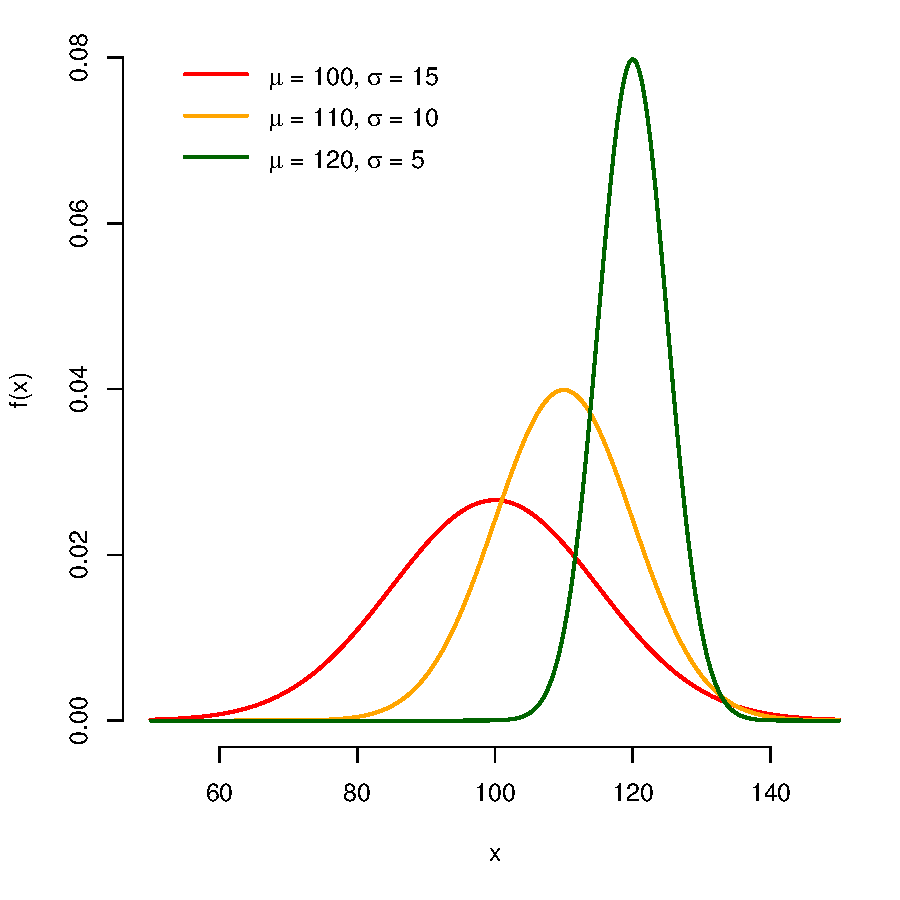
\includegraphics[width=.6\linewidth]{img/ukazka-obr02.pdf}
\caption{A figure with a plot, not entirely related to anything. If you copy the figures from anywhere, always refer to the original author, ideally by citation (if possible). In particular, this picture --- and many others, also a lot of surrounding code --- was taken from the example bachelor thesis of MFF, originally created by Martin Mareš and others.}
\label{fig:g}
\end{figure}

\begin{figure}
\centering
\tikzstyle{box}=[rectangle,draw,rounded corners=0.5ex,fill=green!10]
\begin{tikzpicture}[thick,font=\sf\scriptsize]
\node[box,rotate=45] (a) {A test.};
\node[] (b) at (4,0) {Node with no border!};
\node[circle,draw,dashed,fill=yellow!20, text width=6em, align=center] (c) at (0,4) {Ugly yellow node.\\Is this the Sun?};
\node[box, right=1cm of c] (d) {Math: $X=\sqrt{\frac{y}{z}}$};
\draw[->](a) to (b);
\draw[->](a) to[bend left=30] node[midway,sloped,anchor=north] {flow flows} (c);
\draw[->>>,dotted](b) to[bend right=30] (d);
\draw[ultra thick](c) to (d);

\end{tikzpicture}
\caption{An example diagram typeset with TikZ.}
\label{fig:schema}
\end{figure}

\begin{algorithm}
\begin{algorithmic}
\Function{ExecuteWithHighProbability}{$A$}
	\State $r \gets$ a random number between $0$ and $1$
	\State $\varepsilon \gets 0.0000000000000000000000000000000000000042$
	\If{$r\geq\varepsilon$}
		\State execute $A$ \Comment{We discard the return value}
	\Else
		\State print: \texttt{Not today, sorry.}
	\EndIf
\EndFunction
\end{algorithmic}
\caption{Algorithm that executes an action with high probability. Do not care about formal semantics in the pseudocode --- semicolons, types, correct function call parameters and similar nonsense from `realistic' languages can be safely omitted. Instead make sure that the intuition behind (and perhaps some hints about its correctness or various corner cases) can be seen as easily as possible.}
\label{alg:w}
\end{algorithm}

\section{Extra typesetting hints}

Do not overuse text formatting for highlighting various more or less parts of your sentences; if an idea cannot be communicated without formatting, the sentence probably needs rewriting anyway.

Most importantly, do \underline{not} overuse bold text, which is designed to literally \textbf{shine from the page} to be the first thing that catches the eye of the reader. More precisely, use bold text only for `navigation' elements that need to be seen first, such as headings, list item names, and figure numbers.

Use underline only in dire necessity, such as in the previous paragraph where it was inevitable to ensure that the reader remembers to never typeset boldface text manually again.

Use \emph{emphasis} to highlight the first occurrences of important terms that the reader should notice. The feeling the emphasis produces is, roughly, ``Oh my --- what a nicely slanted word! Surely I expect it be important for the rest of the thesis!''

Finally, never draw a vertical line (e.g., in a table or around figures), ever. Vertical lines outside of the figures are ugly.
\fi
